% LaTeX Template for Project Report, Version 2.0
% (Abstracted from a Major Project Report at CSED, NIT Calicut but can be
% modified easily to use for other reports also.)
%
% Released under Creative Commons Attribution license (CC-BY)
% Info: http://creativecommons.org/licenses/by/3.0/
%
% Created by: Kartik Singhal
% BTech CSE Batch of 2009-13
% NIT Calicut
% Contact Info: kartiksinghal@gmail.com
%
% It is advisable to learn the basics of LaTeX before using this template.
% A good resource to start with is http://en.wikibooks.org/wiki/LaTeX/
%
% All template fields are marked with a pair of angular brackets e.g. <title here>
% except for the ones defining citation names in ref.tex.
%
% Empty space after chapter/section/subsection titles can be used to insert text.
%
% Just compile this file using pdflatex after making all required changes.

\documentclass[12pt,a4paper]{report}
\usepackage[pdftex]{graphicx} %for embedding images
\usepackage{url} %for proper url entries
\usepackage[bookmarks, colorlinks=false, pdfborder={0 0 0}, pdftitle={Project Report}, pdfauthor={Anwar Mohamed}, pdfsubject={project report}, pdfkeywords={artificial intelligence}]{hyperref} %for creating links in the pdf version and other additional pdf attributes, no effect on the printed document
%\usepackage[final]{pdfpages} %for embedding another pdf, remove if not required

\usepackage{listings}
\usepackage{color}

\definecolor{dkgreen}{rgb}{0,0.6,0}
\definecolor{gray}{rgb}{0.5,0.5,0.5}
\definecolor{mauve}{rgb}{0.58,0,0.82}

\lstset{frame=none,
  aboveskip=3mm,
  belowskip=3mm,
  showstringspaces=false,
  columns=flexible,
  basicstyle={\small\ttfamily},
  numbers=none,
  numberstyle=\tiny\color{gray},
  keywordstyle=\color{blue},
  commentstyle=\color{dkgreen},
  stringstyle=\color{mauve},
  breaklines=none,
  breakatwhitespace=true,
  tabsize=4,
}

\begin{document}
\renewcommand\bibname{References} %Renames "Bibliography" to "References" on ref page

%include other pages
\begin{titlepage}

\begin{center}

\textup{\small {\bf Term Project} \\ Report}\\[0.2in]

% Title
\Large \textbf {Tic-Tac-Toe Game}\\[0.5in]

       \small \emph{Submitted in fulfillment of\\
        the requirements of the term project of}
        \vspace{.2in}

       {\bf Artificial Intelligence Course}\\[0.5in]

% Submitted by
\normalsize Submitted by \\
\normalsize Anwar Mohamed - 2491 \\


\vfill

% Bottom of the page

\includegraphics[width=0.18\textwidth]{./foe-logo}\\[0.1in]
\Large{Department of Computer and Communications Engineering}\\
\normalsize
\textsc{Faculty of Engineering - Alexandria University}\\
Alexandria, Egypt\\
\vspace{0.2cm}
Winter Semester 2016

\end{center}

\end{titlepage}


\pagenumbering{roman} %numbering before main content starts
\tableofcontents

\newpage
\pagenumbering{arabic} %reset numbering to normal for the main content

\addtolength{\topmargin}{-1.0in}
\textheight 9.5in

\chapter{Problem Definition}

You are required to implement a tic-tac-toe game using alpha-beta pruning where a user plays against the computer. \\

You are not expected to create a graphical user interface; The game could have a command line interface, but the user must have a way to place an X (or an O) where ever it is possible to do so. But if you think GUI will make it easier for you to test the game, then feel free to use it. \\

Tic-tac-toe is a game with a score of zero, which means that if both players play optimally, no one should win.\\

If you were able to beat the computer (even if it was rare), then this means that your implementation of minimax alpha-beta is incorrect. Every game you play against the computer should end either with a tie or with the computer winning.
 %objective changed to problem definition
\chapter{Introduction}

\section{Perfect Game of Tic Tac Toe}

To begin, let's start by defining what it means to \emph{play a perfect game of tic tac toe}: \\ 

If I play perfectly, every time I play I will either win the game, or I will draw the game. Furthermore if I play against another perfect player, I will always draw the game. How might we describe these situations quantitatively? Let's assign a score to the "\emph{end game conditions}:"

\begin{itemize}
	\itemsep-0.5em 
	\item I win, hurray! I get 10 points!
    \item I lose, shit. I lose 10 points (because the other player gets 10 points).
    \item I draw, whatever. I get zero points, nobody gets any points.
\end{itemize}

To apply this, let's take an example from near the end of a game, where it is my turn. I am X. My goal here, obviously, is to maximize my end game score.\\

\begin{center}
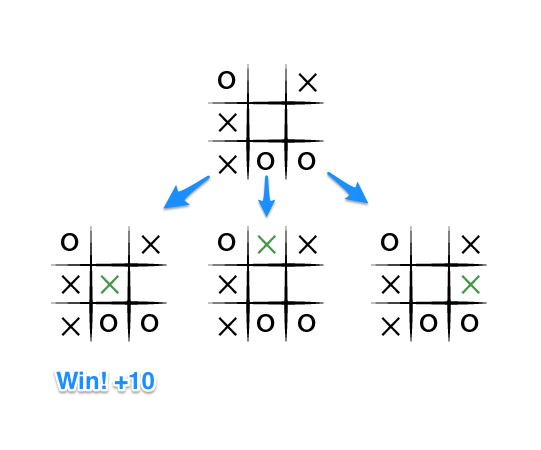
\includegraphics[width=1.1\textwidth]{./a-contrived-end-state-for-a-tic-tac-toe-game}
\end{center}

If the top of this image represents the state of the game I see when it is my turn, then I have some choices to make, there are three places I can play, one of which clearly results in me wining and earning the 10 points. If I don't make that move, O could very easily win. And I don't want O to win, so my goal here, as the first player, should be to pick the maximum scoring move. \\

What do we know about O? Well we should assume that O is also playing to win this game, but relative to us, the first player, O wants obviously wants to chose the move that results in the worst score for us, it wants to pick a move that would minimize our ultimate score. Let's look at things from O's perspective, starting with the two other game states from above in which we don't immediately win: \\

\begin{center}
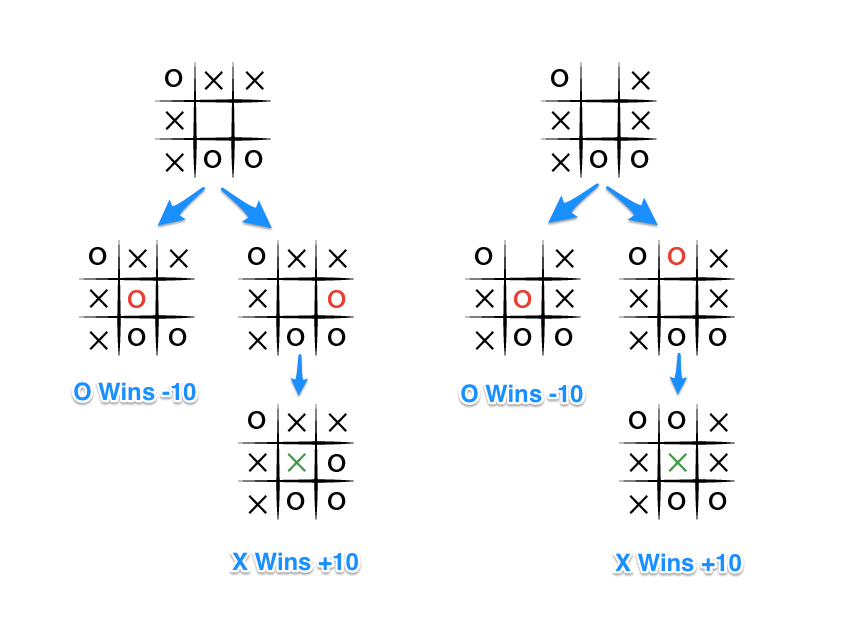
\includegraphics[width=1.1\textwidth]{./a-move-tree-from-the-perspective-of-the-other-player-o}
\end{center}

The choice is clear, O would pick any of the moves that result in a score of -10.

\subsection{Minimax Algorithm}

The key to the Minimax algorithm is a back and forth between the two players, where the player whose "turn it is" desires to pick the move with the maximum score. In turn, the scores for each of the available moves are determined by the opposing player deciding which of its available moves has the minimum score. And the scores for the opposing players moves are again determined by the turn-taking player trying to maximize its score and so on all the way down the move tree to an end state. \\

A description for the algorithm, assuming X is the "turn taking player," would look something like: 

\begin{itemize}
	\itemsep-0.5em 
	\item If the game is over, return the score from X's perspective.
	\item Otherwise get a list of new game states for every possible move.
	\item Create a scores list.
	\item For each of these states add the minimax result of that state to the scores list.
	\item If it's X's turn, return the maximum score from the scores list.
	\item If it's O's turn, return the minimum score from the scores list.
\end{itemize}

\begin{lstlisting}
def minimax(depth, player)
  if gameover || depth == 0
    return calculated_score
  end
  children = all legal moves for player
  if player is AI (maximizing player)
    best_score = -infinity
    for each child
      score = minimax(depth - 1, opponent)
      if (score > best_score)
        best_score = score
      end
      return best_score
    end
  else #player is minimizing player
    best_score = +infinity
    for each child
      score = minimax(depth - 1, player)
      if (score < best_score)
        best_score = score
      end
      return best_score
    end
  end
end

#then you would call it like
minimax(2, computer)
\end{lstlisting}

\begin{center}
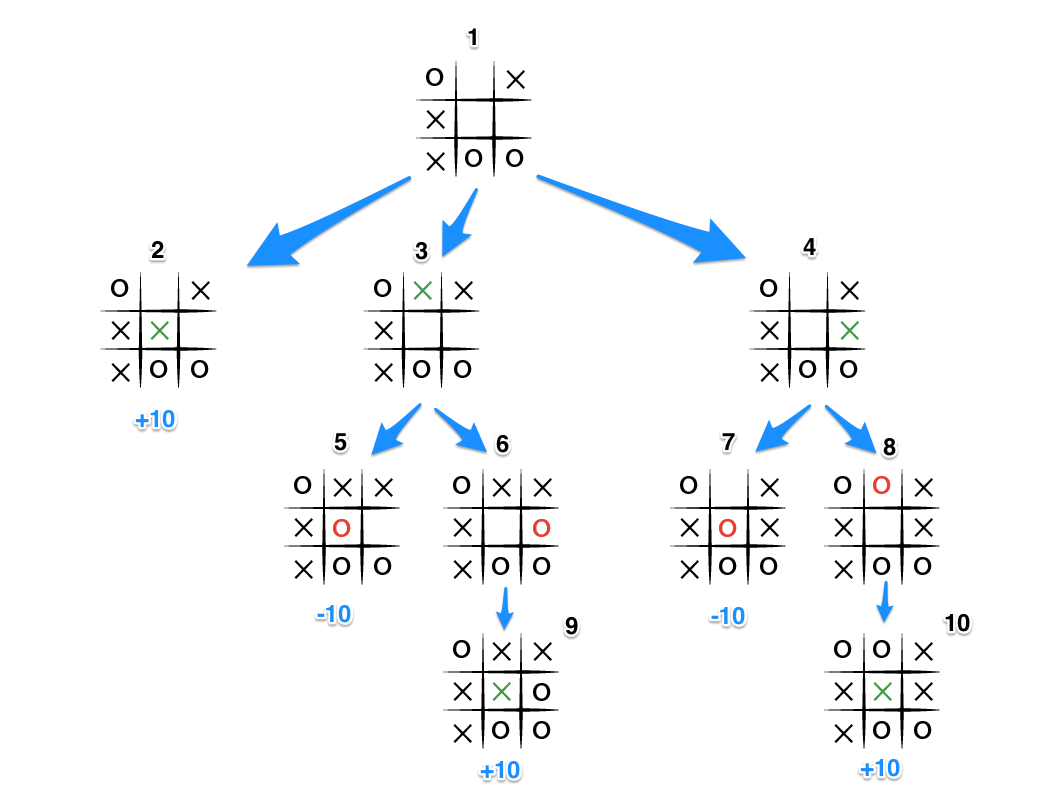
\includegraphics[width=0.9\textwidth]{./full-minimax-move-tree}
\end{center}

\subsection{Alpha-Beta Pruning}

There’s a different algorithm that makes Minimax better, called Alpha-beta pruning. This eliminates paths that are worse than paths that have already been evaluated. Therefore, you have to store a few more values: alpha, which holds the maxmimum score for the maximum path, and beta, which holds the minimum score for the minimum path. You throw away a path when its alpha value is \textgreater= the beta value. \\

\begin{center}
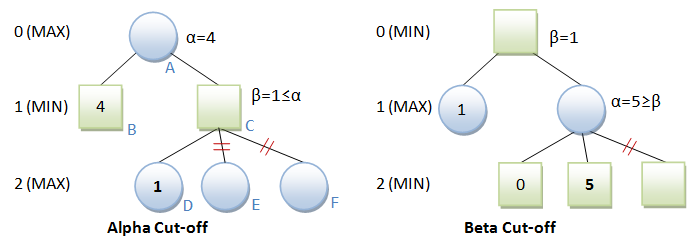
\includegraphics[width=1.1\textwidth]{./GameTTT_alphabeta}
\end{center}

\begin{lstlisting}
def minimax(depth, player, alpha, beta)
  if gameover || depth == 0
    return calculated_score
  end
  children = all legal moves for player
  if player is AI (maximizing player)
    for each child
      score = minimax(depth - 1, opponent, alpha, beta)
      if (score > alpha)		alpha = score	end
      if alpha >= beta     	break			end
      return alpha
    end
  else #player is minimizing player
    best_score = +infinity
    for each child
      score = minimax(depth - 1, player, alpha, beta)
      if (score < beta)		beta = score		end
      if alpha >= beta		break			end
      return beta
    end
  end
end

#then you would call it like
minimax(2, computer, -inf, +inf)
\end{lstlisting} %literature survey included in this
\chapter{Work Done}

\section{Java Implementaion}

I have implemented a simple tic-tac-toe game in Java that utilizes alpha-beta pruning so that the computer can play against computer users. The structure of the game is as following:

\begin{itemize}
	\itemsep-0.5em 
	\item TicTacToe, the driver class for the game.
	\item GameFrame, the graphical user interface class.
	\item GameController, the logic implementaion class.
\end{itemize}

I have added the ability to change the level of difficulty of the game, so there are {\bf Easy}, {\bf Medium} and {\bf Hard} levels.

\section{Game Testing}

\begin{center}
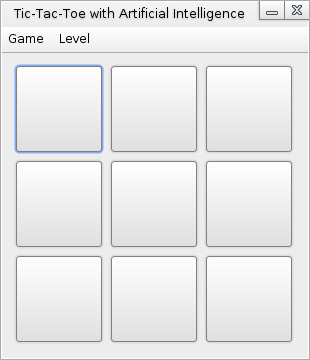
\includegraphics[width=0.45\textwidth]{./game1}
\hspace*{0.1em}
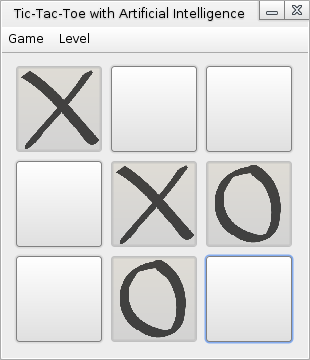
\includegraphics[width=0.45\textwidth]{./game2}

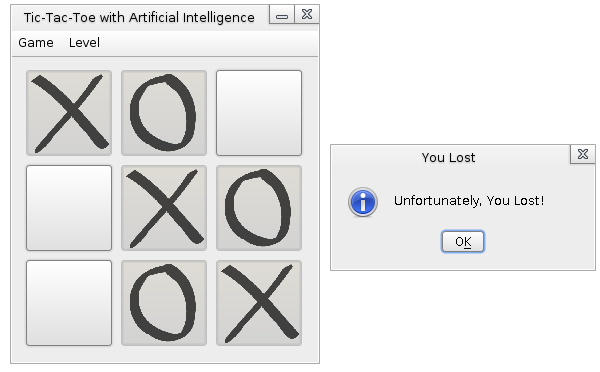
\includegraphics[width=0.9\textwidth]{./game3}
\vspace*{0.3em}

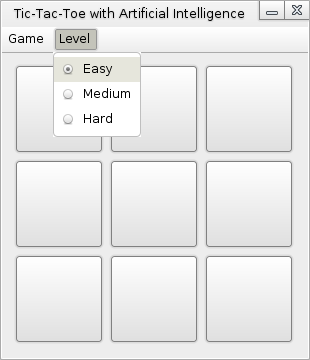
\includegraphics[width=0.45\textwidth]{./game4}
\hspace*{0.1em}
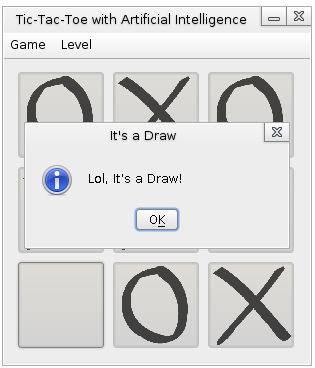
\includegraphics[width=0.45\textwidth]{./game5}

\end{center}
\cleardoublepage
%\pagebreak
\phantomsection
\addcontentsline{toc}{chapter}{References}
\begin{thebibliography}{99}

\bibitem{citation-1}Tic Tac Toe: Understanding The Minimax Algorithm,\ \url{http://neverstopbuilding.com/minimax}

\bibitem{citation-2}Solving Tic-Tac-Toe, Part II: A Better Way,\ \url{http://catarak.github.io/blog/2015/01/07/solving-tic-tac-toe/}

\end{thebibliography}


\end{document}
